%\documentclass{article}

%\usepackage{tikz}
%\usepackage[utf8]{inputenc}
%\usepackage[ngerman]{babel}
%\usepackage{color}
%\usepackage[a4paper,lmargin={2cm},rmargin={2cm},
%tmargin={2.5cm},bmargin = {2.5cm}]{geometry}
%\usepackage{amssymb}
%\usepackage{amsmath}
%\usepackage{graphicx}
%\usepackage{multicol}
%\usepackage{amsthm}

%\newtheorem*{defi*}{Definition}
%\newtheorem*{defi2*}{Definition}

%\begin{document}
%\begin{multicols*}{2}

% \newcommand{\norm}[1]{\left\lVert#1\right\rVert}

\subsection{Norm und Skalarprodukt}

\begin{Def}
$\norm{v}$ ist eine Norm im Vektorraum $V$ falls
\begin{enumerate}
\item 
\begin{enumerate}
\item $\norm{v} \geq 0$ für alle $v \in V$
\item $\norm{v} = 0$ nur für $v = 0$
\end{enumerate}
\item $\norm{u+v} \leq \norm{u} + \norm{v}$ für alle $v \in V$
\item $\norm{\lambda v} = |\lambda| \norm{v}$ für alle $\lambda \in \mathbb{R}$ und $v \in V$
\end{enumerate}
\end{Def}

Die zweite Ungleichung nennt man auch Dreiecksungleichung.
In Worte gefasst ergeben sich die folgenden Eigenschaften: Eine Norm kann nie negativ sein, ist die Norm 0 bedeutet das, dass der Vektor der Nullvektor ist. Wenn man zwei Vektoren
addiert, ist die Norm des resultierenden Vektors kleiner oder gleich der Summe der Normen der beiden Ausgangsvektoren. Außerdem ist die
Norm eines Vektors, der mit einem reellen Faktor multipliziert wurde, gleich dem Produkt aus der Norm des Vektors und dem 
Betrag des Faktors.

\begin{Def}
$f:V\times V \rightarrow\mathbb{R}$ ist ein Skalarprodukt, wenn\\
\begin{enumerate}
\item $\left\langle  \alpha u + \beta v, w\right\rangle = \alpha \left\langle  u,w\right\rangle + \beta \left\langle  v,w\right\rangle $ (Bilinearität)
\item $\left\langle  u,v\right\rangle = \left\langle  v,u\right\rangle $ für alle $u,v \in V$
\item $\left\langle  v,v\right\rangle \geq 0$ mit $\left\langle  v,v\right\rangle = 0$ nur für $v = 0$
\end{enumerate}
\end{Def}
Wir können ein Skalarprodukt im euklidischen Raum $\mathbb{R}$ mit
\begin{equation}
\left\langle u,v\right\rangle  = u_1 v_1 + \dots + u_n v_n
\label{skal}
\end{equation}
definieren. An der ausgeschriebenen Form lässt sich überprüfen, ob es sich dabei wirklich um ein Skalarprodukt handelt. Hierbei kann  $\left\langle \alpha u + \beta v, w\right\rangle $ zu $\sum_{i=1}^n (\alpha u_i + \beta v_i)w_i$ umgeformt werden. Durch das Ausmultiplizieren der Produkte erhalten wir die Form $\sum_{i=1}^n \alpha u_i w_i + \beta v_i w_i$. Wenn wir daraus nach zwei Summen sortieren und die Summanden mit $\alpha$ von denen mit $\beta$ trennen, können wir die beiden Faktoren ausklammern und gelangen zu der aus der Definition geforderten Form $\alpha \left\langle u,w\right\rangle  + \beta \left\langle v,w\right\rangle $.
Die zweite Bedingung können wir mit dem Kommutativgesetz beweisen, wenn wir dieses auf die ausgeschriebene Form anwenden.
Für die dritte Bedingung bekommen wir $\sum_{i=1}^n v_i v_i = \sum_{i=1}^n v_i^2$. Da durch das Quadrieren keiner der Summanden kleiner als 0 werden kann und auch nur für $v_i = 0$ genau 0 werden kann, ist auch diese Bedingung erfüllt.

\begin{dsafigure}
\centering
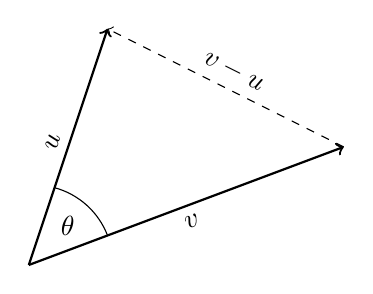
\begin{tikzpicture}
\coordinate (A) at (0,0);
\coordinate (B) at (4,1.5);
\coordinate (C) at (1,3);
\draw[thick, ->] (A) -- (B) node[pos=0.5,sloped,below]{$v$};
\draw[thick, ->] (A) -- (C) node[pos=0.5,sloped, above]{$u$};
\draw[dashed, ->] (B) -- (C) node[pos=0.5,sloped, above]{$v-u$};
\draw (1,0.375) arc (21:75:1);
\node[] at (45:0.7) {$\theta$};
\end{tikzpicture}
\caption {Anwendung des Kosinussatzes}
\label{Kosinussatz}
\end{dsafigure}

Da grundsätzlich $\langle v,v\rangle  = \norm{v}^2$ gilt, kann über die Abbildung \ref{Kosinussatz} auch die Aussage getroffen werden, dass $\norm{v-u}^2 = \left\langle v-u,v-u\right\rangle $. Mit der Bilinearität des Skalarproduktes und der eben getroffenen Aussage können wir die Gleichung zu 
$\lVert v-u\rVert ^2 = \lVert v\rVert ^2 - 2\left\langle v,u\right\rangle  + \lVert u\rVert ^2$
umformen.
Zusätzlich folgt aus dem Kosinussatz, dass $\norm{v-u}^2 = \norm{u}^2 + \norm{v}^2 - 2 \norm{u} \norm{v} \cos\theta$. Setzt man beide Terme gleich, gelangt man über einige wenige Umformungen zu der Form $\left\langle u,v\right\rangle  = \norm{u} \norm{v} \cos\theta$, was ebenfalls eine Möglichkeit ist, das Skalarprodukt darzustellen.
Aus dieser Gleichung ergibt sich direkt die Cauchy-Schwarz Ungleichung. Da sich der Betrag des Kosinus nur zwischen 0 und 1 bewegt, gilt
\begin{equation}
\left\langle u,v\right\rangle  \leq \norm{u} \norm{v}.
\label{cauchy}
\end{equation}

Eine häufig genutzte Norm ist die Euklidische Norm, welche durch $\norm{v}_2 = \sqrt{v_1^2 + \dots + v_n^2}$ definiert ist und auch durch die obrige Definition des Skalarproduktes \eqref{skal} induziert wird.

Die erste und die dritte Bedingung aus der Definition für eine Norm zeigen sich aus der ausgeschriebenen Form der Euklidischen Norm. Da alle Komponenten dabei quadriert werden und die Wurzel gezogen wird, muss die erste Bedingung stimmen. Ein Faktor $\lambda$, der ebenfalls quadriert in der Wurzel steht kann aus der Summe ausgeklammert werden und als Faktor vor die Wurzel gelangen. Der Betrag ergibt sich dabei daraus, dass $\lambda$ nach dem Vorgang nur positiv sein kann, auch wenn es zuvor negativ war.

Um zu beweisen, dass die Dreiecksungleichung $\norm{u+v} \leq\norm{u} + \norm{v}$  gilt,benötigen wir die Dreiecksungleichung für reelle Zahlen und die Cauchy-Schwarz Ungleichung. Wir gehen dabei von der quadrierten Form des linken Terms aus und erhalten
\begin{align*}
\norm{u+v}^2 &= |\left\langle u+v,u+v\right\rangle|\\
&\leq |\left\langle u,u\right\rangle| + 2|\left\langle u,v\right\rangle| + |\left\langle v,v\right\rangle|\\
&\leq \norm{v}^2 + 2\norm{u} \norm{v} + \norm{v}^2\\
&= (\norm{u} + \norm{v})^2.
\end{align*}

Man sieht sofort, dass der Ausgangsterm kleiner oder gleich dem Ergebnis ist, womit bewiesen ist, dass die Euklidische Norm eine Norm ist.

%\end{multicols*}
%\end{document}
